\chapter{Парсинг изображений CAPTCHA и их предобработка для создания датасета}

\section{Парсинг реальных CAPTCHA с различных web-ресурсов}

Большинство предобученных моделей компьютерного зрения, таких как YOLOv8, обучены на датасете COCO~\cite{COCO}, содержащем изображения высокого качества с чёткими контурами и однозначной аннотацией объектов. Однако CAPTCHA с изображениями имеют принципиально иные характеристики: они могут включать в себя размытие, наложенные артефакты, искажения, шумы, повторяющиеся элементы и искусственно пониженное разрешение. Всё это снижает эффективность использования стандартных датасетов и моделей, не адаптированных под такие условия.

Для обеспечения высокой точности в задаче автоматического решения CAPTCHA необходимо подготовить собственный набор данных, приближённый к реальным условиям использования. Наиболее эффективным методом является автоматизированный парсинг изображений CAPTCHA, представленных на веб-сайтах, использующих визуальные CAPTCHA-решения, такие как Google reCAPTCHA v2.

Использование реальных CAPTCHA, собранных в автоматическом режиме, имеет ряд преимуществ по сравнению с синтетической генерацией данных:

\begin{enumerate}
    \item изображения содержат разнообразные сцены, освещение, углы обзора и уровни шума, что положительно влияет на способность модели к обобщению;
    \item присутствует большое количество уникальных объектов на фоне, в том числе в частично перекрытых и смазанных вариантах;
    \item отсутствует необходимость в ручной генерации изображений и создании дополнительных искажений для повышения реалистичности;
    \item возможно извлекать текстовые инструкции к CAPTCHA, что позволяет соотносить каждое изображение с требуемым классом.
\end{enumerate}

Для парсинга CAPTCHA был реализован автоматизированный сценарий взаимодействия с браузером с использованием библиотеки Selenium~\cite{Selenium}. Данный подход позволяет воспроизвести действия пользователя при работе с CAPTCHA, обходя при этом ручной ввод. Для обеспечения стабильной работы и масштабируемости процесса применялась браузерная автоматизация через WebDriver (в частности, ChromeDriver).

Функциональность парсера включает следующие ключевые этапы:

\begin{enumerate}
    \item поиск iframe-элемента, содержащего чекбокс <<Я не робот>>, и эмуляция клика по нему для инициирования визуальной CAPTCHA;
    \item ожидание загрузки CAPTCHA и извлечение изображения с заданием (включая его URL или пиксельный снимок);
    \item извлечение информации о структуре сетки (количество строк и столбцов), на которую разбито изображение CAPTCHA;
    \item получение текста задания, содержащего имя объекта (например, <<выберите все изображения с мотоциклами>>), для последующего использования в аннотации данных.
\end{enumerate}

Типичная CAPTCHA представляет собой изображение, разделённое на сетку из 3×3 или 4×4 ячеек, каждая из которых может содержать фрагмент сцены. При этом пользователю предлагается выбрать ячейки, в которых присутствует объект заданного класса. Процесс парсинга может быть представлена блок-схемой на рис.~\ref{fig:captcha-flow}.

\begin{figure}[H]
    \centering
    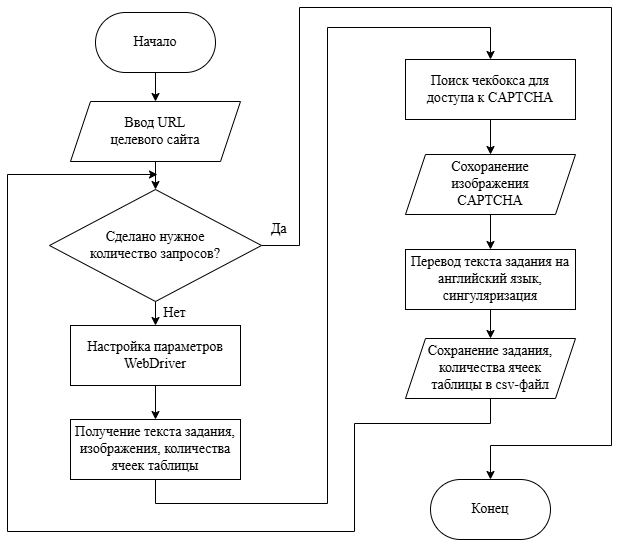
\includegraphics[width=0.65\textwidth]{imgs/image_captcha_flow.png}
    \caption{Блок-схема процесса парсинга CAPTCHA.}
    \label{fig:captcha-flow}
\end{figure}
\vspace{-0.5cm}

Полученные изображения и метаданные (включая текст задания и параметры сетки) используются для формирования обучающего датасета, пригодного для дообучения модели YOLOv8 в задачах классификации и сегментации объектов.

\section{Предварительная обработка изображений датасета}

После получения достаточного количества изображений для составления датасета необходимо провести их предварительную обработку и разметку. Это один из самых важных этапов работы, поскольку от качества разметки напрямую зависит точность и эффективность последующей работы модели.

Для корректной работы модели YOLO требуется создать иерархическую структуру папок, в которой изображения и соответствующие метки будут разделены на тренировочную и валидационную выборки. Стандартная структура включает следующие директории:

\begin{enumerate}
    \item Директория train -- содержит тренировочную выборку:
    \begin{enumerate}
        \item images -- изображения;
        \item labels -- метки к изображениям.
    \end{enumerate}
    \item Директория val -- содержит валидационную выборку:
    \begin{enumerate}
        \item images -- изображения;
        \item labels -- метки к изображениям.
    \end{enumerate}
\end{enumerate}

Набор классов, пути к выборкам и параметры конфигурации задаются в YAML-файле, который передается при обучении модели. Содержимое такого файла для данной модели:

\begin{code}
\captionof{listing}{\label{code:train-captcha}Параметры конфигурации для обучения модели}
\vspace{-0.5cm}
{\small
\inputminted[mathescape,linenos,frame=lines,breaklines]{yaml}{code/train_captcha.yaml}
}
\end{code}
\vspace{-0.4cm}

Для создания меток используется инструмент CVAT (Computer Vision Annotation Tool) -- многофункциональное веб-приложение с поддержкой аннотации объектов с помощью полигонов, прямоугольников и других форм. CVAT позволяет экспортировать разметку напрямую в формат, совместимый с YOLO~\cite{CVAT}.

Поскольку CAPTCHA-изображения часто содержат объекты с нечёткими контурами, наложением и визуальными искажениями, особенно важно использовать ручную точную разметку, а не ограничиваться автоматическими методами. Выделение объектов должно проводиться как можно точнее, с учётом геометрии контуров. На рисунке ниже представлен пример изображения с размеченными объектами:

\begin{figure}[H]
    \centering
    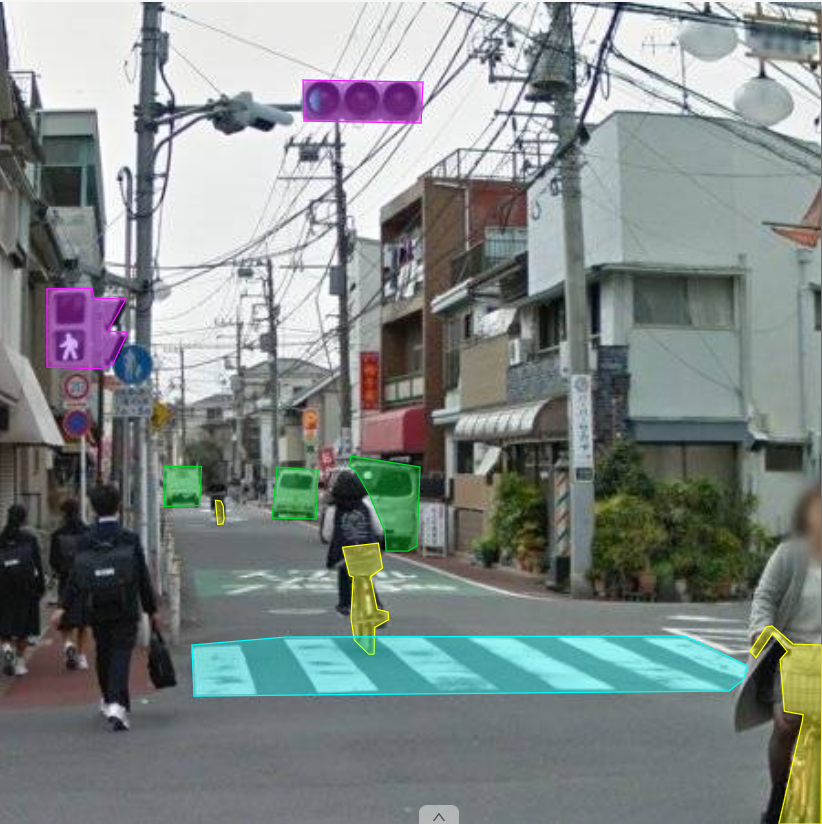
\includegraphics[width=0.9\linewidth]{imgs/captcha-poligons.png}
    \caption{Пример разметки изображения с тестовой CAPTCHA.}
    \label{fig:mask-captcha}
\end{figure}
\vspace{-0.5cm}

Кроме того, разметка позволяет учесть сразу несколько объектов разных классов на одном изображении, что особенно характерно для CAPTCHA, где в одной сетке могут одновременно находиться, например, автомобили и автобусы. Такой подход положительно влияет на обобщающую способность модели.

В случае, если количество данных по отдельным классам окажется недостаточным, можно дополнительно использовать методы аугментации: вращение, масштабирование, искажение цвета и контраста. Однако при хорошо организованном парсинге и разметке зачастую удается обойтись без аугментации.
